\section{ResNet}
\label{resnet}
ResNet (abbreviazione di \textit{residual network}) è il nome di un'ampia categoria di reti neurali convoluzionali profonde, caratterizzate dall'utilizzo di particolari blocchi di layer detti \textit{residual blocks}, ideati per risolvere alcuni problemi delle reti molto profonde.
Le reti ResNet propriamente dette sono state introdotte da un gruppo di ricercatori Microsoft nel 2015 nel paper \cite{resnet}. Presentate nell'edizione del 2015 della \textit{ILSVRC} e risultate vincitrici con uno strabiliante errore \textit{top-5} su dataset ImageNet 3.57\% (più basso di quello umano, stimato a 5\%), queste reti sono considerate tutt'oggi lo stato dell'arte nell'ambito delle reti neurali convoluzionali profonde.\\

Nell'ambito dei problemi di visione artificiale proposti nella ILSVRC, in quegli anni cominciava ad essere evidente (\cite{googlenet},\cite{verydeep}) che la profondità delle reti neurali era di fondamentale importanza per il miglioramento delle prestazioni delle reti su dataset di grandi dimensioni, quali il database ImageNet (par. \ref{imagenet}).
L'ovvia conseguenza di questa osservazione è stato il tentativo di aumentare progressivamente il numero di layer delle reti neurali, rendendole sempre più profonde e complesse, con l'aggravarsi di ostacoli già noti (quali ad esempio il problema della scomparsa del gradiente, par. \ref{vanishingGradientProblem}) e il presentarsi di nuovi (un problema di degradazione esposto per la prima volta in \cite{highway}, e descritto nel seguito):
ResNet nasce per dare soluzione a questi problemi:

\begin{itemize}

\item Il problema della scomparsa e dell'esplosione del gradiente è attenuato da un insieme di strategie già messe in campo in precedenza, su tutte la \textit{batch normalization} (par. \ref{batchNormalization}) introdotta dal team dei creatori di GoogLeNet \cite{batchNorm}.

\item Quando una rete molto profonda comincia a convergere verso un minimo della funzione costo (in fase di addestramento), si presenta un problema di degradazione: al crescere della profondità della rete la sua \textit{training accuracy} tende a saturarsi e in seguito prende a degradarsi rapidamente, come mostrato in fig. \ref{fig:degradation}.

\begin{figure}[h!]
\centering
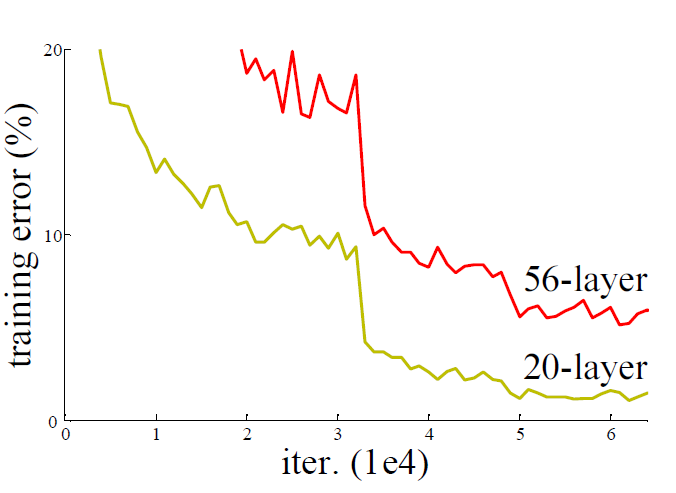
\includegraphics[width=0.5\textwidth]{degradation.png}
\caption{Problema di degradazione della \textit{training accuracy} su CNN "standard" da 20 e 56 layer rispettivamente. La rete più profonda ha un \textit{training error} più alto. \cite{resnet} per più dettagli.}
\label{fig:degradation}
\end{figure}

È un problema inaspettato e diverso rispetto all'\textit{overfitting} (che interessa solamente il valore della \textit{validation accuracy}) e indica che la difficoltà nell'ottimizzare una rete convoluzionale "standard" cresce con la sua profondità. ResNet aggira questo problema con l'introduzione dei \textit{residual blocks} (par. \ref{residualBlock})

\end{itemize}

\subsection{\textit{Batch Normalization}}
\label{batchNormalization}
La \textit{Batch Normalization} è il nome di una tecnica introdotta dal team di GoogLeNet e ad oggi ampiamente utilizzata che permette un addestramento più veloce e stabile delle reti neurali profonde \cite{batchNorm}.

Essa consiste in una normalizzazione delle attivazioni di un certo layer, generalmente prima di passare gli stessi ad un'eventuale funzione di attivazione ed in seguito all'eventuale layer successivo.

L'algoritmo per l'applicazione della tecnica è riportato di seguito\\

\begin{adjustwidth}{3em}{0em}

\textbf{Input:} Attivazioni $\mathbf{x}=\{x_1,\dots,x_m\};$\\
\phantom{\textbf{Input:} }Parametri da imparare: $\gamma, \beta$\\
\noindent \textbf{Output:} Attivazioni normalizzate $y_i = BN_{\gamma,\beta}(x_i)\}$

\begin{align}
& \mu_{\mathbf{x}}\leftarrow\frac{1}{m}\sum_{i=1}^m x_i && \text{// media delle attivazioni} \notag\\
& \sigma^2_{\mathbf{x}}\leftarrow\frac{1}{m}\sum_{i=1}^m \left(x_i-\mu_{\mathbf{x}}\right)^2 && \text{// varianza delle attivazioni} \notag\\
& \widehat{x_i}\leftarrow\frac{x_i-\mu_{\mathbf{x}}}{\sqrt{\sigma^2_{\mathbf{x}}+\varepsilon}} && \text{// normalizzazione} \notag\\
& y_i\leftarrow\gamma\widehat{x_i}+\beta\equiv BN_{\gamma,\beta}(x_i)\} && \text{// scale e offset} \notag
\label{eq:batchNorm}
\end{align}

\end{adjustwidth}

I parametri $\gamma$ e $\beta$, chiamati rispettivamente \textit{scale} e \textit{offset}, sono imparati dalla rete in fase di addestramento. La loro funzione è far sì che le attivazioni normalizzate non siano necessariamente a media nulla e varianza unitaria (in modo da poter variare arbitrariamente l'intervallo utilizzato nel dominio della eventuale funzione di attivazione successiva alla normalizzazione).\\

Nonostante sia oggi ampiamente utilizzata, le ragioni dell'efficienza della \textit{batch normalization} sono ancora scarsamente comprese. Ricerche recenti \cite{realBatchNorm} hanno mostrato che ciò che questa tecnica produce non è una riduzione dell'\textit{internal covariate shift} (la variabilità statistica dei mini-batch usati, che ad ogni iterazione causa uno spostamento del punto di minimo della funzione costo), come affermato dagli autori del paper originale \cite{batchNorm}, ma è una "lisciatura" (\textit{smoothing}) della funzione costo, che induce un comportamento più stabile e predicibile dei gradienti, comportando un addestramento più veloce.

In ogni caso, la \textit{batch normalization} si è rivelata efficace per l'attenuazione del problema della scomparsa del gradiente o della sua esplosione; inoltre si è verificato che il suo utilizzo porta anche ad una maggiore regolarizzazione dei parametri dell'apprendimento, migliorando la robustezza all'overfitting.

Questa tecnica ha permesso quindi la progettazione di reti sempre più profonde, ma non elimina tutti i problemi collegati all'estrema profondità dell'architettura (persiste ad esempio il problema di degradazione descritto nel precedente paragrafo).

\subsection{Residual blocks}
\label{residualBlock}
Il principale contributo di ResNet nell'ambito del deep learning è sicuramente l'introduzione dei cosiddetti \textit{residual blocks} e delle \textit{shortcut connections} ("scorciatoie") per risolvere il problema di degradazione in precedenza descritto. In fig. \ref{fig:residualBlock} è mostrato uno schema generale dell'oggetto in esame.

\begin{figure}[h!]
\centering
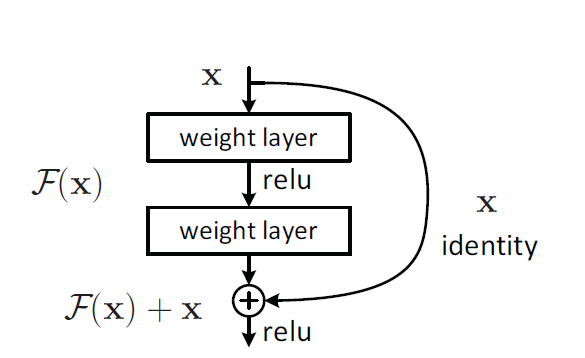
\includegraphics[width=0.6\textwidth]{residualBlock.png}
\caption{\textit{Residual block} con \textit{shortcut identity mapping}. Si noti che i particolari layer di questo blocco sono arbitrari.}
\label{fig:residualBlock}
\end{figure}

Invece di sperare che un dato blocco di layer non lineari contigui impari ad approssimare una certa funzione $\mathcal{H}(\mathbf{x})$ desiderata, si decide di creare una "scorciatoia" (propriamente \textit{shortcut connection}) che connette l'input $\mathbf{x}$ e l'output del blocco (vd. fig. \ref{fig:residualBlock}); in questo modo il blocco deve imparare ad approssimare non più la funzione desiderata $\mathcal{H}(\mathbf{x})$ ma una funzione residuale $\mathcal{F}(\mathbf{x})\coloneqq\mathcal{H}(\mathbf{x})-\mathbf{x}$. In definitiva il blocco addestrato darà in output la funzione $\mathcal{F}(\mathbf{x})+\mathbf{x}$.\\

Per introdurre la motivazione che spinge alla progettazione di questo particolare blocco, facciamo il seguente esperimento.
Consideriamo una generica rete neurale con $n$ layer. Costruiamo una rete neurale con $n+k$ layer che ha come layer iniziali gli $n$ layer della prima rete e i rimanenti $k$ layer approssimano funzioni identità ($\mathcal{F}(\mathbf{x})=\mathbf{x}$). L'esistenza di una seconda rete più profonda della prima ma con le stesse prestazioni indica che una rete più profonda dovrebbe avere un \textit{training error} più basso o almeno uguale a quella meno profonda. Gli esperimenti in \cite{resnet} hanno mostrato tuttavia che non conosciamo nessun algoritmo di ottimizzazione che permetta almeno di eguagliare il \textit{training error} della prima rete addestrando la seconda rete descritta (almeno in un tempo non lungo). Questa è una delle forme in cui si manifesta il \textit{degradation problem} discusso in precedenza.

L'idea dei \textit{residual blocks}, peraltro non nuova e già utilizzata in precedenza (ad es. \cite{highway}), è basata sull'ipotesi degli autori - corroborata dall'esperimento di cui sopra - che le reti neurali abbiano difficoltà ad approssimare attraverso i loro tanti layer non lineari una funzione lineare (come appunto l'identità $\mathcal{f}(\mathbf{x})=\mathbf{x}$); in altre parole, viene ipotizzato che sia più facile per un blocco di layer imparare la funzione residua rispetto alla funzione originale. Ecco perché si decide di fornire direttamente l'input in uscita con una \textit{shortcut connection}, evitando al blocco lo sforzo di dover imparare a mappare un'identità.\\

Le straordinarie prestazioni raggiunte dalle reti ResNet estremamente profonde confermano che l'intuizione degli autori era corretta. Senza aver aggiunto complessità computazionale (escludendo le trascurabili somme dovute alle \textit{shortcut connections}) resta così risolto il problema di degradazione della \textit{training accuracy}.

\subsection{Architettura di ResNet-18}
ResNet-18 è una rete neurale convoluzionale profonda addestrata sul dataset ImageNet (par. \ref{imagenet}). La rete accetta in input immagini $224\times 224$ ed è composta da 18 layer parametrizzati, di cui un layer convoluzionale iniziale con filtro $7\times 7$ (seguito da batch normalization, ReLU e max pooling), altri 16 layer convoluzionali $3\times 3$ raccolti a due a due in 8 \textit{residual blocks} (descritti di seguito) e infine  un layer completamente connesso (preceduto da ReLU e average pooling) dalle cui 1000 attivazioni si calcola la distribuzione di probabilità per le 1000 classi di ImageNet, per mezzo della funzione softmax.
Il particolare \textit{residual block} adoperato in ResNet-18 è del tipo mostrato in figura \ref{fig:residualBlockResnet18}

\begin{figure}[H]
\centering
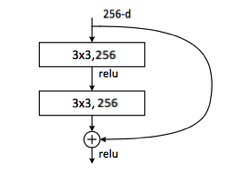
\includegraphics[width=0.4\textwidth]{residualBlockResnet18.png}
\caption{Uno degli otto \textit{residual blocks} di ResNet-18}
\label{fig:residualBlockResnet18}
\end{figure}

Il ramo che ospita i layer non lineari si compone delle seguenti operazioni:

\begin{itemize}
\item Convoluzione $3\times 3$\footnote{il numero di filtri di convoluzione, e quindi la profondità del volume di output, è riportata per ciascun \textit{residual block} in fig. \ref{fig:architetturaResnet18} e in fig. \ref{fig:confrontoResnet}}
\item Batch Normalization
\item ReLU
\item Convoluzione $3\times 3$
\item Batch Normalization
\end{itemize}

Inoltre, il ramo che realizza la \textit{shortcut connection} si compone eventualmente di una convoluzione $1\times 1$ seguita da batch normalization per garantire che il volume di attivazioni che attraversa la "scorciatoia" abbia dimensioni confrontabili con il volume uscente dal ramo che ospita i layer non lineari. Questa eventualità è rappresentata in fig. \ref{fig:architetturaResnet50} con un arco tratteggiato.\\

L'architettura di ResNet-18 è riportata schematicamente nella figura \ref{fig:architetturaResnet18} e in forma tabellare, in confronto con ResNet-50, in fig. \ref{fig:confrontoResnet} nel prossimo sottoparagrafo.

\subsection{Architettura di ResNet-50}
ResNet-50 è una variante più profonda di ResNet-18. Come la sua omologa meno profonda, questa rete accetta in input immagini $224\times 224$; essa è composta da 50 layer parametrizzati, di cui un layer convoluzionale iniziale con filtro $7\times 7$ (seguito da \textit{batch normalization}, ReLU e max pooling), altri 48 layer convoluzionali di varie dimensioni raccolti a gruppi di tre in 16 \textit{residual blocks} (descritti di seguito) e infine  un layer completamente connesso con le usuali 1000 attivazioni.
Il particolare \textit{residual block} adoperato in ResNet-50 è del tipo mostrato in figura \ref{fig:residualBlockResnet50}

\begin{figure}[H]
\centering
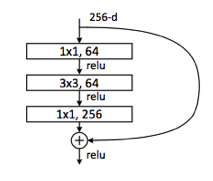
\includegraphics[width=0.4\textwidth]{residualBlockResnet50.png}
\caption{Uno dei sedici \textit{residual blocks} di ResNet-50}
\label{fig:residualBlockResnet50}
\end{figure}

Il ramo che ospita i layer non lineari si compone delle seguenti operazioni:

\begin{itemize}
\item Convoluzione $1\times 1$
\item Batch Normalization
\item ReLU
\item Convoluzione $3\times 3$
\item Batch Normalization
\item ReLU
\item Convoluzione $1\times 1$
\item Batch Normalization
\end{itemize}

Inoltre, il ramo che realizza la \textit{shortcut connection} si compone eventualmente di una convoluzione $1\times 1$ seguita da batch normalization per garantire che il volume di attivazioni che attraversa la "scorciatoia" abbia dimensioni confrontabili con il volume uscente dal ramo che ospita i layer non lineari. Questa eventualità è rappresentata in fig. \ref{fig:architetturaResnet50} con un arco tratteggiato.\\

L'evidente differenza rispetto al \textit{residual block} di ResNet-18 è motivata dalla premura di dover mantenere basso il tempo necessario ad addestrare la rete. Le convoluzioni $3\times 3$ sono computazionalmente costose, pertanto in reti molto profonde non si possono prevedere tutti \textit{residual blocks} ciascuno operante due convoluzioni $3\times 3$. Si decide allora di modificare il \textit{residual block} usato: si decide di operare un'unica convoluzione $3\times 3$ per blocco, preceduta e seguita da una convoluzione $1\times 1$ (par. \ref{conv1x1}) per rispettivamente ridurre e ripristinare la profondità del volume di attivazioni su cui la convoluzione $3\times 3$ lavora, abbassando così il costo computazionale associato all'addestramento di ciascun \textit{residual block}.\\

L'architettura di ResNet-50 è riportata schematicamente nella figura \ref{fig:architetturaResnet50} e in forma tabellare, in confronto con quella di ResNet-18, in fig. \ref{fig:confrontoResnet} seguente.

\begin{figure}[h!]
\centering
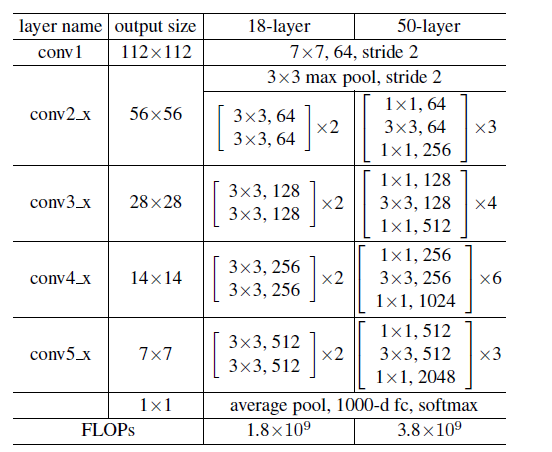
\includegraphics[width=0.9\textwidth, height=\textheight, keepaspectratio]{architetturaResnet.png}
\caption{Le architetture di ResNet-18 e ResNet-50 a confronto}
\label{fig:confrontoResnet}
\end{figure}

\begin{figure}[h]
  \begin{minipage}[b]{0.475\textwidth}
  \centering
    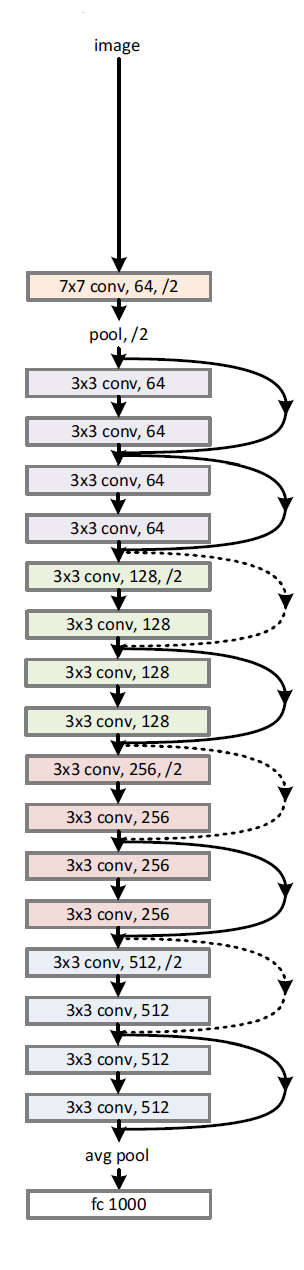
\includegraphics[width=\textwidth, height=\textheight, keepaspectratio]{architetturaResnet18.png}
    \caption{Architettura di ResNet-18}
    \label{fig:architetturaResnet18}
  \end{minipage}
  \hfill
  \begin{minipage}[b]{0.475\textwidth}
  \centering
    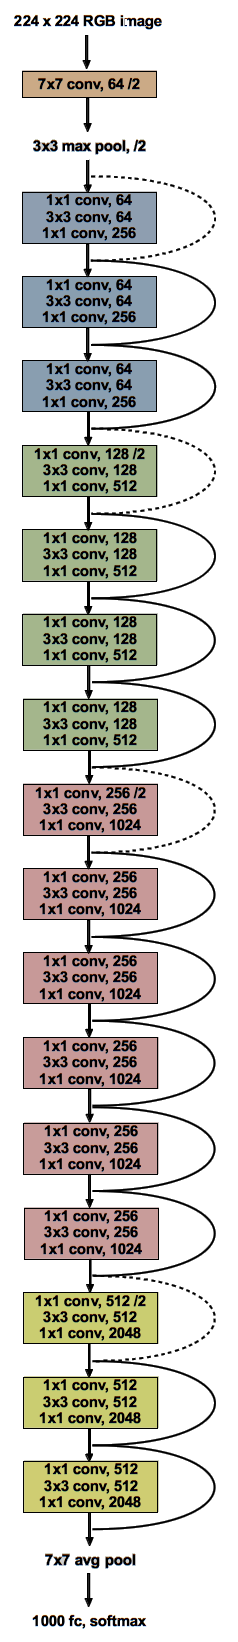
\includegraphics[width=\textwidth, height=\textheight, keepaspectratio]{architetturaResnet50.png}
    \caption{Architettura di ResNet-50}
    \label{fig:architetturaResnet50}
  \end{minipage}
\end{figure}

\subsection{Data Augmentation}
\label{augmentationResnet}
Come d'uso, anche ResNet-18 e ResNet-50 adoperano una strategia di \textit{data augmentation} per ridurre l'overfitting al training set di ImageNet.
Ogni immagine è ridimensionata con il suo lato più corto estratto casualmente dall'intervallo $[256,480]$ e mantenendo l'\textit{aspect ratio}. Viene ritagliata una \textit{patch} (ritaglio) $224\times 224$ casuale dall'immagine così ridimensionata e ad ogni canale della patch viene sottratta la media dei valori R, G e B del dataset ImageNet (similmente ad AlexNet, par. \ref{augmentationAlexnet}). Il ritaglio è eventualmente capovolto orizzontalmente (50\% di probabilità)

\subsection{Addestramento di ResNet-18 e ResNet-50}
Le reti ResNet-18 e ResNet-50 sono state addestrate sul database ImageNet usando la discesa stocastica del gradiente con momento = 0.9, mini-batch = 256 e decadimento dei pesi (\textit{weight decay}) = 0.0001. Il \textit{learning rate} iniziale è 0.1, ed è soggetto ad una strategia di \textit{annealing} che lo riduce di un fattore 10 ogniqualvolta il \textit{training error} si stabilizza. Il numero massimo di iterazioni di addestramento è $6\times 10^5$. I pesi sono inizializzati secondo il metodo descritto in \cite{weightsResnet}, creato dagli stessi autori di ResNet. Dettagli più specifici sulla fase di addestramento di ResNet-18 e ResNet-50 possono essere trovati nel paper originale \cite{resnet}.